%
% LaTeX report template 
%
\documentclass[a4paper,10pt]{article}
\usepackage{graphicx}
\usepackage{amsmath}
\usepackage{amssymb}
\usepackage[italian]{babel}
\usepackage[utf8]{inputenc}
\usepackage[margin=1.25in]{geometry}
\graphicspath{{../img/}}

%
\begin{document}
%

   
   \title{{\large Universita' degli Studi di Padova \\ } {\normalsize Corso di laurea triennale in Ingegneria Informatica}\\ \vspace{1.8cm} \textbf{ Relazione 3\textsuperscript{a} simulazione SPICE}}

   \author{Giacomo Camposampiero, matricola 1187180}
          
   \date{21 gennaio 2021}

   \maketitle
      
   \vspace{1.8cm}   
   \renewcommand{\contentsname}{Indice}      
   \tableofcontents
   
   \newpage
  
\section{Esercizio primo}
Il circuito in Figura \ref{fig:ckt1} rappresenta un amplificatore operazionale CMOS a due stadi. L'uscita single-ended del primo stadio è rappresentata dalla tensione nel punto D$_2$. L’uscita del secondo stadio è la tensione $v_o$ ai drain di Q$_6$-Q$_7$. La corrente I$_{ref}$ = 90 $\mu$A; $V_{Tn}$ = 0.7 V, k’$_n$ = 160 $\frac{\mu A}{V^2}$, $V_{An}$ = $V_{Ap}$= 10V, $V_{Tp}$=-0.8 V, k’$_p$=40 $\frac{\mu A}{V^2}$, V$_{DD}$= V$_{SS}$ = 2.5V. Le dimensioni dei transistor sono specificate nella Tabella \ref{tabelladim}.
\begin{figure}[h!]
  	\centering
 	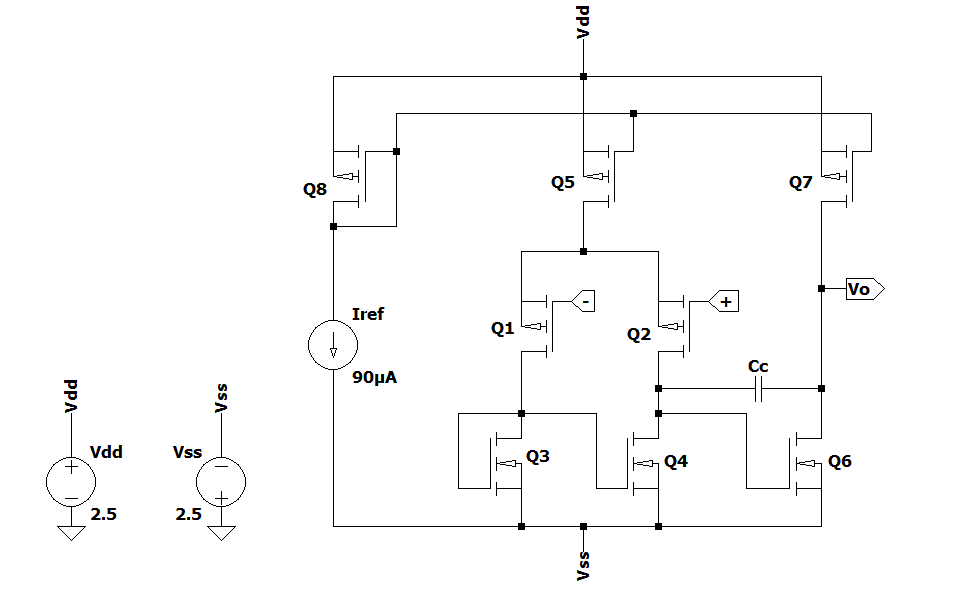
\includegraphics[width=0.9\linewidth]{ckt1.png}
  	\caption{Schema elettrico dell'amplificatore operazionale CMOS a due stadi.}
  	\label{fig:ckt1}
\end{figure}

\begin{table}[h!]
\begin{center}
\begin{tabular}{ |c|c|c|c|c|c|c|c|c| } 
 \hline
   Transistore & $Q_1$ & $Q_2$ & $Q_3$ & $Q_4$ & $Q_5$ & $Q_6$ & $Q_7$ & $Q_8$ \\ 
  \hline
 W/L & $20/0.8$ & $20/0.8$ & $5/0.8$ & $5/0.8$ & $40/0.8$ & $10/0.8$ & $40/0.8$ & $40/0.8$ \\ 
 \hline
\end{tabular}
 \caption{Dimensioni transistor.}
\label{tabelladim}
\end{center}
\end{table}

\subsection{Calcolare il punto di polarizzazione di ogni transistor: I$_{DQ}$, V$_{GSQ}$, V$_{DSQ}$, trascurando l'effetto di modulazione della lunghezza di canale}
Come prima cosa, calcoliamo il parametro di transconduttanza k$_n$ per tutti i MOS di diverse dimensioni
\begin{align*}
\left( k_p=\frac{2mA}{V^2} \right)_{40/0.8} \quad  \left( k_p=\frac{1mA}{V^2} \right)_{20/0.8} \quad \left( k_n=\frac{2mA}{V^2} \right)_{10/0.8} \quad\left( k_n=\frac{1mA}{V^2} \right)_{5/0.8}
\end{align*}
Cominciamo a calcolare il punto di polarizzazione di ogni transistor dal PMOS Q$_8$. In questo caso la corrente di drain $I_{SDQ}$ è fissata dal generatore ideale di corrente $I_{\mathit{ref}}$, per cui $I_{SDQ}=90\mu A$. Gate e drain del transistor sono cortocircuitati e, di conseguenza, il MOSFET si trova in saturazione. Dalla relazione della corrente di drain in saturazione, troviamo le tensioni
\begin{equation*}
V_{SGQ}= V_{SDQ} = V_{ov} + \left| V_{Tp} \right| = \sqrt{\frac{2 \cdot I_{SDQ}}{K_p}} + 0.8 = 1.1\,V 
\end{equation*}
Per cui le tensioni $V_{G,8}=V_{D,8}=1.4\, V$, dove $V_{G,8}$ è la tensione con cui sono pilotati i transistor $Q_7$ e $Q_5$. Avendo entrambi questi ultimi source collegato a $V_{DD}$, troviamo che entrambi specchiano la stessa corrente $I_{SDQ}$ e (nell'ipotesi di saturazione, da verificare una volta trovato $V_{SDQ}$) entrambi hanno la stessa tensione $V_{SGQ}$, rispettivamente
\begin{equation*}
I_{SDQ}=90\, \mu A \qquad \qquad V_{SGQ}=1.1\,V
\end{equation*}
Conoscendo la corrente di drain del transistor $Q_5$ possiamo notare che, per simmetria del circuito, la corrente che scorre nei due transistor $Q_1$ e $Q_2$ è
\begin{equation*}
I_{SDQ,1} = I_{SDQ,2} = \frac{I}{2} = 45\, \mu A
\end{equation*}
dove I corrisponde alla corrente $I_{SDQ,5}$. Nell'ipotesi in cui i due MOS sono in saturazione (da verificare), dalla relazione della corrente riusciamo a ricavare la tensione 
\begin{equation*}
V_{SGQ}= V_{SDQ} = V_{ov} + \left| V_{Tp} \right| = \sqrt{\frac{2 \cdot I_{SDQ}}{K_p}} + 0.8 = 1.1\,V 
\end{equation*}
Da questa differenza di potenziale possiamo ricavare il potenziale al drain di $Q_5$ e, di conseguenza, la tensione $V_{SDQ}$ del transistor $Q_5$, $V_{SDQ}=V_{DD}-V_D=1.4\,V$. L'ipotesi di saturazione è quindi verificata, in quanto
\begin{equation*}
V_{SDQ,5} = 1.4\,V > V_{SGQ,5} - \left| V_{tp} \right| = 0.3\,V
\end{equation*} 
Noto il punto di polarizzazione dei transistor $Q_1$ e $Q_2$, risulta facile trovare quello dei transistor $Q_3$ e $Q_4$. La corrente che scorre nei due è infatti la stessa ($I_{DSQ}=45 \mu A$) e $Q_3$ si trova sempre in saturazione in quanto drain e gate sono cortocircuitati. In queste condizioni, ricaviamo dalla relazione della corrente la tensione
\begin{equation*}
V_{GSQ}= V_{DSQ} = \sqrt{\frac{2 \cdot I_{DSQ}}{K_n}} + 0.7 = 1\,V
\end{equation*}
Siamo in grado quindi di verificare la condizione di saturazione dei transistor $Q_1$ e $Q_2$, ora che è nota la tensione di drain di questi ultimi
\begin{equation*}
V_{SDQ}= 2.6\,V > V_{SGQ} - \left| V_{tp} \right| = 0.3\,V
\end{equation*}
Infine, troviamo la polarizzazione del transistor $Q_6$. La tensione di gate risulta essere $V_G=-1.5\,V$, per cui $V_{GSQ}=1\,V$. La corrente di drain in questo caso è la stessa del transistor $Q_7$, ovvero 90$\mu$A. La tensione $V_{DSQ}$ è l'unica tensione che non si riesce a ricavare esplicitamente dai calcoli. Possiamo però ricavare un intervallo all'interno della quale è compresa, a partire dalle condizioni di funzionamento in saturazione sui transistor $Q_6$ e $Q_7$.
\begin{equation*}
\begin{cases}	
	V_{SDQ,7} > V_{SGQ,7} - \left| V_{Tp} \right|  \Rightarrow -V_{D,7} < -V_{G,7} - \left| V_{Tp} \right|\\ 
	V_{DSQ,6} > V_{GSQ,6} - V_{Tn} \Rightarrow V_{D,6} > V_{G,6} - V_{Tn}
\end{cases}
\end{equation*}
da cui otteniamo
\begin{equation}
\label{valorisat}
-2.2\,V < V_D < 2.2\,V
\end{equation}
Riassumendo, i valori di polarizzazione dei transistor sono riportati in Tabella \ref{tabellapol}.
\begin{table}[h!]
\begin{center}
\begin{tabular}{ |c|c|c|c|c|c|c|c|c| } 
 \hline
   Transistor & $Q_1$ & $Q_2$ & $Q_3$ & $Q_4$ & $Q_5$ & $Q_6$ & $Q_7$ & $Q_8$ \\ 
 \hline
 $\left| I_{DSQ} \right|$ & $45\mu A$ & $45\mu A$ & $45\mu A$ & $45\mu A$ & $90\mu A$ & $90\mu A$ & $90\mu A$ & $90\mu A$ \\
 $\left| V_{GSQ} \right|$ & $1.1\,V$ & $1.1\,V$ & $1\,V$ & $1\,V$ & $1.1\,V$ & $1\,V$ & $1.1\,V$ & $1.1\,V$ \\ 
 \
 $\left| V_{DSQ} \right|$ & $2.6\,V$ & $2.6\,V$ & $1\,V$ & $1\,V$ & $1.4\,V$ & $-$ & $-$ & $1.1\,V$ \\ 
 \hline
\end{tabular}
 \caption{Punto di polarizzazione dei transistor.}
\label{tabellapol}
\end{center}
\end{table}

\newpage
\subsection{Calcolare g$_m$ e r$_o$ per ogni transistor}
Il calcolo dei parametri del modello per piccolo segnale per ogni transistor è riportato di seguito. I calcoli dei parametri per transistor con uguali caratteristiche (stessa $V_{GSQ}$ e transconduttanza) sono stati tra loro raggruppati.\\ \\
Per quanto riguarda i transistor $Q_1$ e $Q_2$, troviamo
\begin{align*}
g_m = k_n \cdot (V_{SGQ}- \left| V_{Tp} \right|) = 0.3\,mS \qquad \qquad \qquad r_o = \frac{V_{Ap}}{I^*_D} = 222\,k\Omega
\end{align*}
Per quanto riguarda i transistor $Q_5$, $Q_7$ e $Q_8$, troviamo
\begin{align*}
g_m = k_n \cdot (V_{SGQ}- \left| V_{Tp} \right|) = 0.6\,mS \qquad \qquad \qquad r_o = \frac{V_{Ap}}{I^*_D} = 111\,k\Omega
\end{align*}
Per quanto riguarda i transistor $Q_3$ e $Q_4$, troviamo
\begin{align*}
g_m = k_n \cdot (V_{GSQ}- V_{Tn}) = 0.3\,mS \qquad \qquad \qquad r_o = \frac{V_{An}}{I^*_D} = 222\,k\Omega
\end{align*}
Per quanto riguarda il transistor $Q_6$, infine, troviamo
\begin{align*}
g_m = k_n \cdot (V_{GSQ}- V_{Tn}) = 0.6\,mS \qquad \qquad \qquad r_o = \frac{V_{An}}{I^*_D} = 111\,k\Omega
\end{align*}

\subsection{Calcolare il guadagno complessivo dell'amplificatore}
Per calcolare il guadagno complessivo dell'amplificatore, iniziamo con il calcolo del guadagno differenziale single-ended del primo stadio dell'amplificatore, ovvero della coppia MOS con carico attivo. Dalla teoria, sappiamo che l'uscita di questo stadio può essere ricavata allo stesso modo dal circuito semplificato ottenuto dalla serie del generatore di corrente pilotato in tensione $G_m v_{id} $ e dalla resistenza $R_o$, dove $G_m$ è la transconduttanza di circuito e $R_o$ la resistenza di uscita dello stadio. In particolare, si può dimostrare che la transconduttanza di circuito equivale a
\begin{equation*}
G_m = g_{m,1} = g_{m,2}
\end{equation*}
La resistenza di uscita al primo stadio è calcolata applicando la tensione di prova $V_x$ al drain di Q$_2$ e Q$_4$, staccando gli ingressi e azzerando tutte le tensioni/correnti continue nel circuito. Ne risulta quindi che la corrente $i_x$ di prova in ingresso all'uscita è
\begin{equation*}
i_x = v_x \cdot \frac{r_{o2} + r_{o4}}{r_{o2}r_{o4}}
\end{equation*}
e la resistenza in uscita R$_o$ è di conseguenza uguale a
\begin{equation*}
\frac{v_x}{i_x} = \frac{r_{o2}r_{o4}}{r_{o2} + r_{o4}} = r_{o2}\, ||\, r_{o4}
\end{equation*}
Il guadagno in tensione del primo stadio (differenziale) può essere quindi calcolato come
\begin{equation}
\label{primog}
A_{v1} = - G_m(r_{o2} \, || r_{o2}) = -\,33.3 \, \frac{V}{V}
\end{equation}
Il secondo stadio è invece un amplificatore a source comune con carico attivo. In questo caso la transconduttanza del secondo stadio G$_m$ coincide con la transconduttanza g$_{m6}$ del transistor Q$_6$. La resistenza in uscita del secondo stadio può essere invece calcolata e coincide con
\begin{equation*}
R_{o}=r_{o6} \, || \, r_{o7}
\end{equation*}
Come nello stadio precedente quindi il guadagno in tensione può essere calcolato come
\begin{equation}
\label{secondog}
A_{v2} = - g_{m6}\,(r_{o6} \, || \, r_{o7}) = -\,33.3 \, \frac{V}{V}
\end{equation}
Il guadagno complessivo, ottenuto unendo (\ref{primog}) e (\ref{secondog}), è dato quindi dal prodotto
\begin{equation}
A_v = A_{v1}A_{v2} = (-33.3)^2 = 1108.89\, \frac{V}{V}
\end{equation}


\subsection{Per quale valore della tensione di uscita Q$_7$ non è più in saturazione? Per quale valore di tensione di uscita Q$_6$ non è più in saturazione?}
I valori di tensione dell'uscita per cui i transistor Q$_6$ e Q$_7$ non sono più in condizione di saturazione sono stati già trovati nella relazione (\ref{valorisat}) al punto 1.1, $-2.2\,V < V_D < 2.2\,V$.

\subsection{Simulare con SPICE il comportamento del circuito, applicando un segnale differenziale puro v$_{id}$ di ampiezza crescente e tracciare il grafico di v$_o$ e v(n4) funzione di v$_{id}$ con v$_{id}$ tra -100 mV e 100 mV}
Per simulare il comportamento del circuito è stato utilizzato il seguente listato SPICE
\begin{quote}
\begin{verbatim}
* Esercizio 1
* alimentazione
Vdd Vdd 0 2.5
Vss Vss 0 -2.5
* current mirror
M8 N1 N1 Vdd Vdd PMOS40
M5 N2 N1 Vdd Vdd PMOS40
Iref N1 Vss 90u
* load
M7 Vo N1 Vdd Vdd PMOS40
* first amp stadium
M1 N3 - N2 Vdd PMOS20
M2 N4 + N2 Vdd PMOS20
M3 N3 N3 Vss Vss NMOS5
M4 N4 N3 Vss Vss NMOS5
* second amp stadium
M6 Vo N4 Vss Vss NMOS10
* capacitor
Cc Vo N4 10p
* input differenziali
Bi1 + 0 V=V(id)/2
Bi2 - 0 V=-V(id)/2
* portanti
Vcm cm 0 AC SINE(0 1m 1k)
Vid id 0 AC SINE(0 {amp} 1k)
* model
.model NMOS5 NMOS LEVEL=1 VTO=0.7 KP=160u W=5u L=0.8u LAMBDA=0.1
.model NMOS10 NMOS LEVEL=1 VTO=0.7 KP=160u W=10u L=0.8u LAMBDA=0.1
.model PMOS20 PMOS LEVEL=1 VTO=-0.8 KP=40u W=20u L=0.8u LAMBDA=0.1
.model PMOS40 PMOS LEVEL=1 VTO=-0.8 KP=40u W=40u L=0.8u LAMBDA=0.1
* richiesta analisi
.step param amp list 100u 500u 1m 2m 10m 50m 100m
.tran 0 1.5m
.backanno
.end
\end{verbatim}
\end{quote}
Il valore dell'ampiezza dell'ingresso differenziale è stato fatto variare all'interno dell'insieme di valori $\{100\, \mu V, 500\, \mu V, 1\, mV, 2\, mV, 10\, mV, 50\, mV, 100\, mV\}$, scelti in modo tale da permettere l'osservazione della tensione ai due nodi per valori di ingresso anche molto diversi tra loro senza appesantire eccessivamente i grafici risultanti. I risultati della simulazione sono riportati in Figura \ref{fig:vidv4} e Figura \ref{fig:vidvo}.\\
\begin{figure}[h!]
  	\centering
 	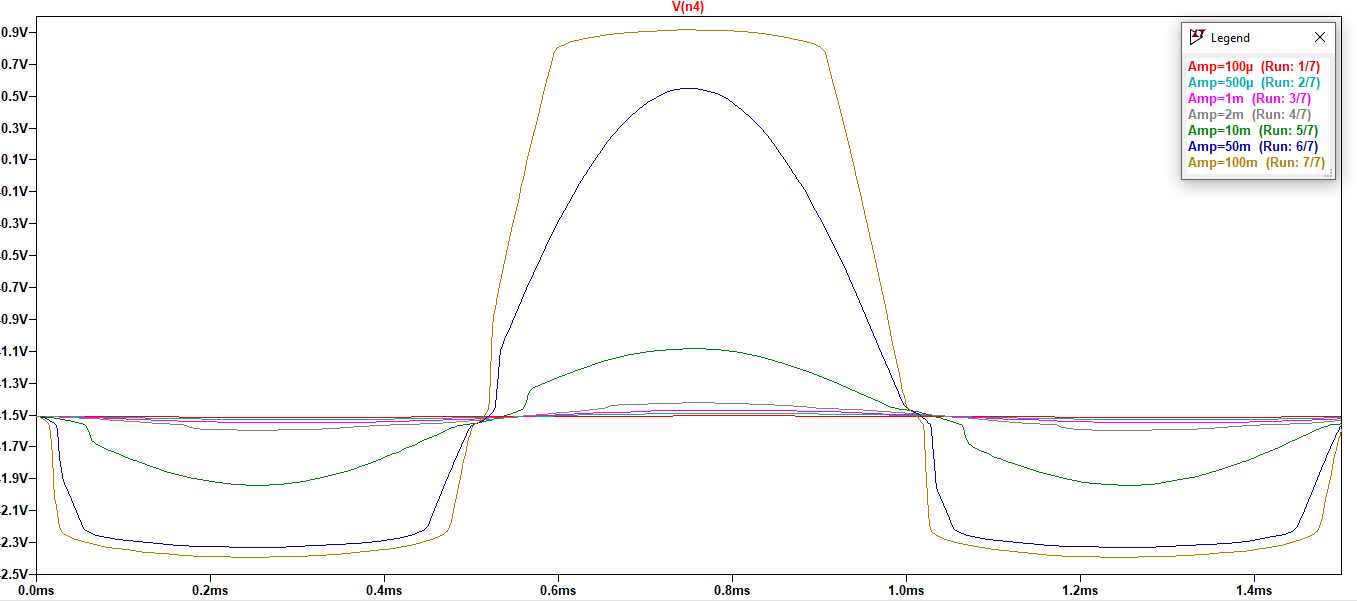
\includegraphics[width=1\linewidth]{es1-5-n41.png}
  	\caption{Tensione in uscita al primo stadio dell'amplificatore.}
  	\label{fig:vidv4}
\end{figure}
\begin{figure}[h!]
  	\centering
 	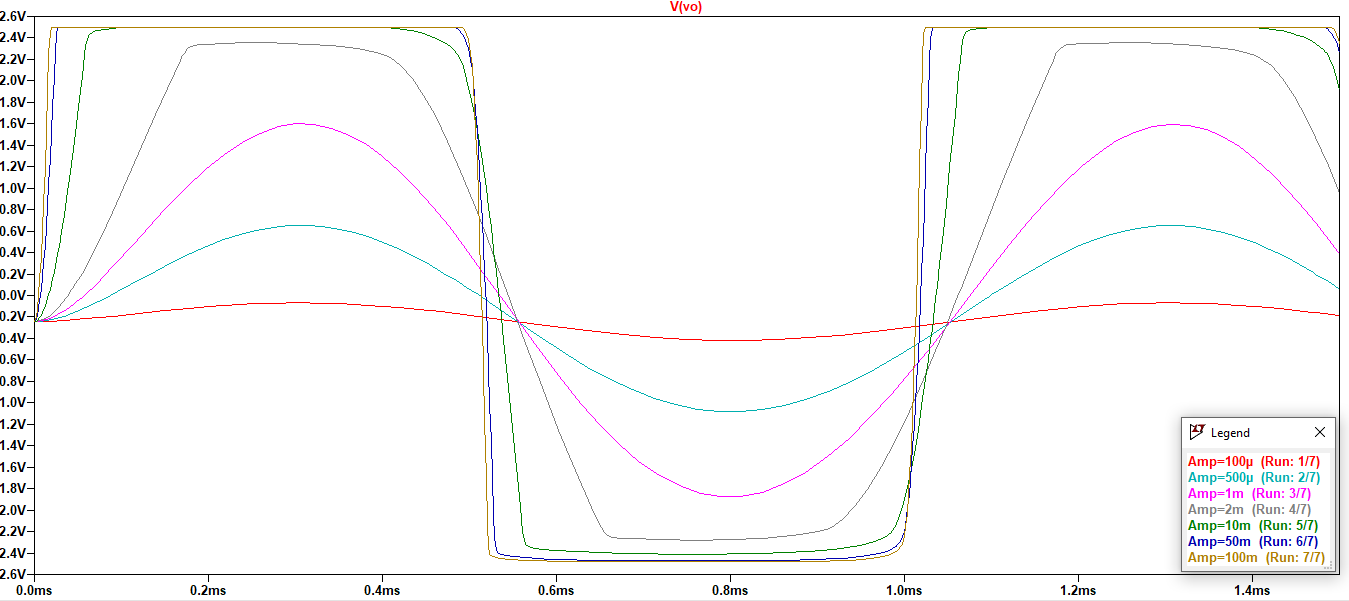
\includegraphics[width=1\linewidth]{es1-5-out1.png}
  	\caption{Tensione in uscita al secondo stadio dell'amplificatore.}
  	\label{fig:vidvo}
\end{figure}

Dai grafici ottenuti è possibile vedere molto chiaramente come i segnali in uscita ai due stadi siano tra loro in opposizione di fase (conseguenza diretta del fatto che i guadagni sono negativi e causano di conseguenza un'inversione del segnale). Inoltre, l'analisi parametrizzata ci permette di osservare in modo chiaro il fenomeno di saturazione delle uscite dei due stati, che avviene nel momento in cui l'ampiezza del segnale amplificato supera la tensione di alimentazione dell'amplificatore stesso. Come ci aspetta, l'uscita del secondo stadio satura per ampiezze di ingresso molto inferiori rispetto al primo stadio. 

\newpage
\subsection{Simulare con SPICE un segnale di modo comune v$_{cm}$ di ampiezza crescente e tracciare il grafico di v(D2) e v$_o$ funzione di v$_{cm}$ con v$_{cm}$ tra -1V e 1V}
Il listato SPICE utilizzato per simulare i comportamenti richiesti sono gli stessi riportati al punto precedente, con l'unica differenza che gli ingressi dell'amplificatore questa volta sono definiti come
\begin{quote}
\begin{verbatim}
Bi1 + 0 V=V(cm)
Bi2 - 0 V=V(cm)
\end{verbatim}
\end{quote}
Le modalità di simulazione rimangono pressocché invariate, con l'unica differenza che l'insieme di valori utilizzati per far variare l'ampiezza del segnale in ingresso diventa $\{1\, mV, 10\, mV, 50\, mV$, $100\, mV, 250\, mV, 500\, mV, 750\, mV, 1\, V \}$. I risultati della simulazione sono riportati in Figura \ref{fig:vcmv4} e Figura \ref{fig:vcmvo}.\\
\begin{figure}[h!]
  	\centering
 	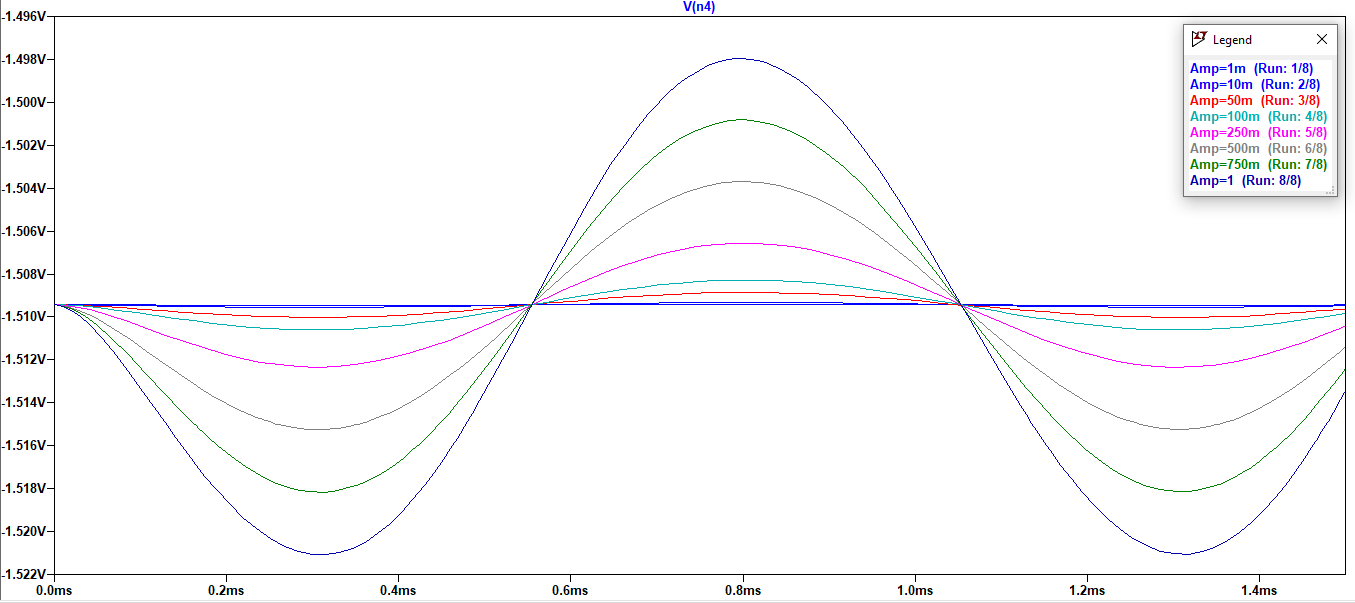
\includegraphics[width=0.9\linewidth]{es1-6-n4.png}
  	\caption{Tensione in uscita al primo stadio dell'amplificatore.}
  	\label{fig:vcmv4}
\end{figure}
\begin{figure}[h!]
  	\centering
 	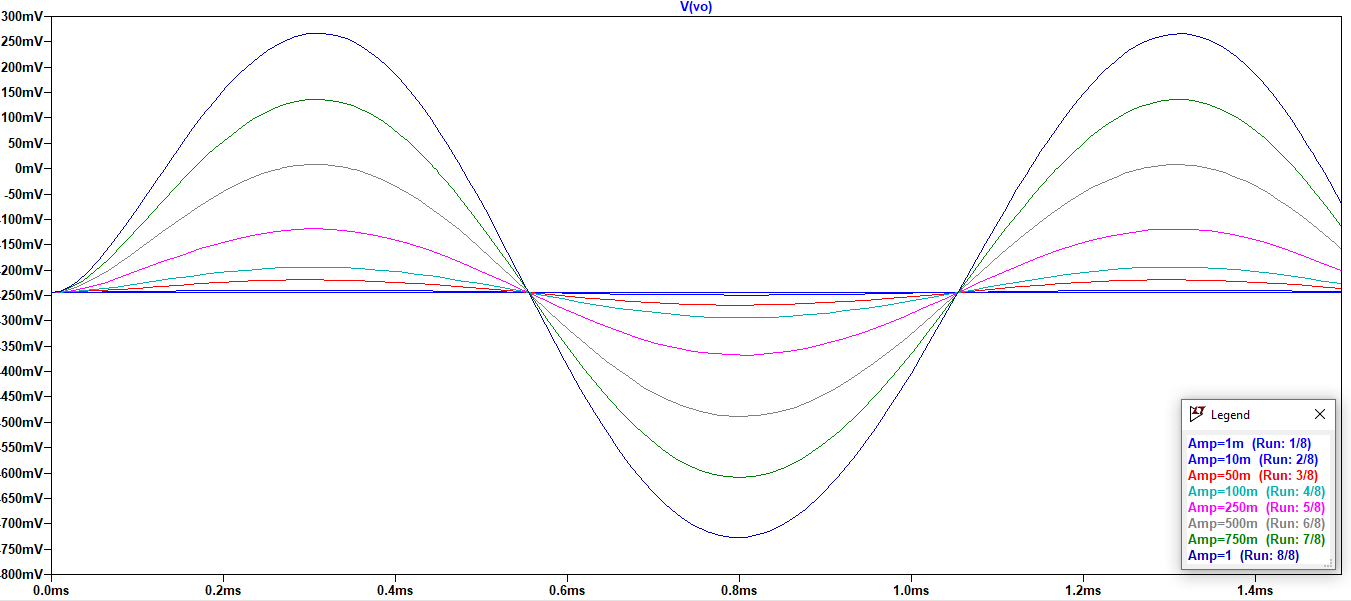
\includegraphics[width=0.9\linewidth]{es1-6-out.png}
  	\caption{Tensione in uscita al secondo stadio dell'amplificatore.}
  	\label{fig:vcmvo}
\end{figure}

Possiamo notare in questo caso che il segnale di modo comune non causa mai saturazione in uscita. I segnali in uscita al primo e secondo stadio dell'amplificatore sono ancora in opposizione di fase (il secondo stadio non è differenziale, per cui amplifica indiscriminatamente qualsiasi segnale; per lo stesso motivo l'ampiezza del segnale in uscita al secondo stadio è maggiore rispetto a quella al primo). Inoltre, è facile dedurre che il guadagno di modo comune del primo stadio è $<<1$.

\newpage
\subsection{Valutare il guadagno differenziale e il guadagno di modo comune dell'amplificatore con SPICE}
Per simulare il comportamento del guadagno complessivo dell'amplificatore, utilizziamo un'analisi in frequenza tra 1 e 100$\,$kHz e segnali in ingresso
\begin{quote}
\begin{verbatim}
Vcm cm 0 AC SINE(0 1m 1k)
Vid id 0 AC SINE(0 1m 1k)
\end{verbatim}
\end{quote}
Le caratteristiche del guadagno differenziale e del guadagno di modo comune sono riportate, rispettivamente, in Figura \ref{fig:gainid} e Figura \ref{fig:gaincm}.\\

\begin{figure}[h!]
  	\centering
 	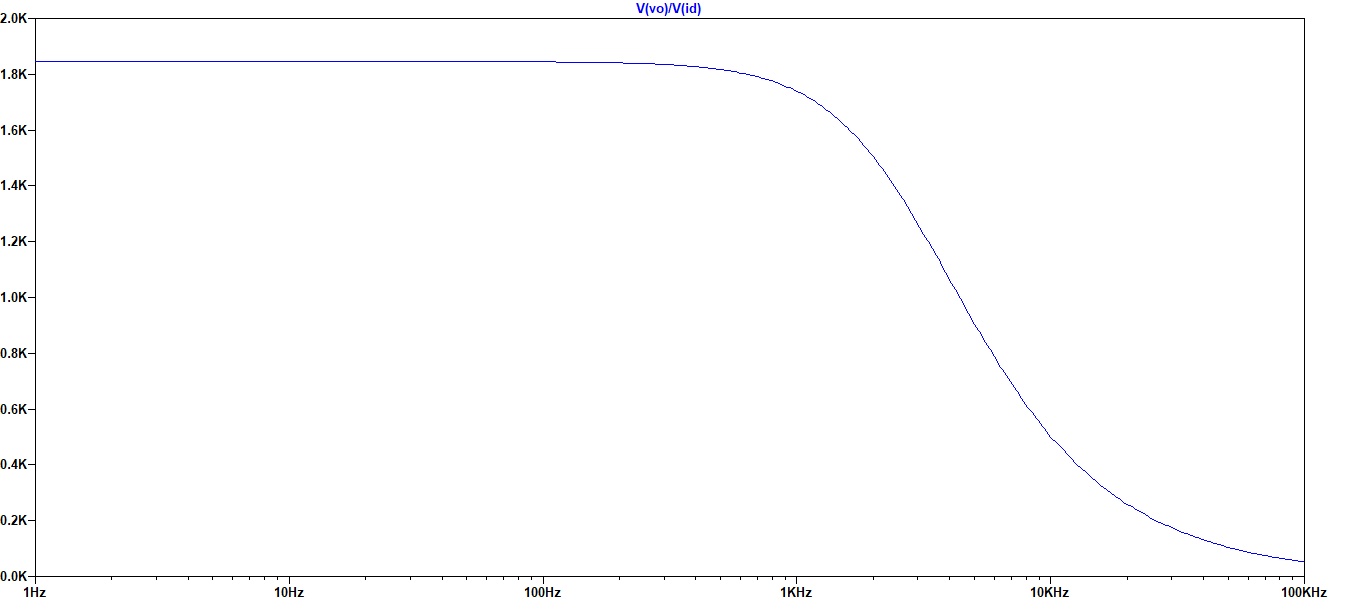
\includegraphics[width=0.9\linewidth]{es1-7-id.png}
  	\caption{Guadagno differenziale complessivo.}
  	\label{fig:gainid}
\end{figure}
\begin{figure}[h!]
  	\centering
 	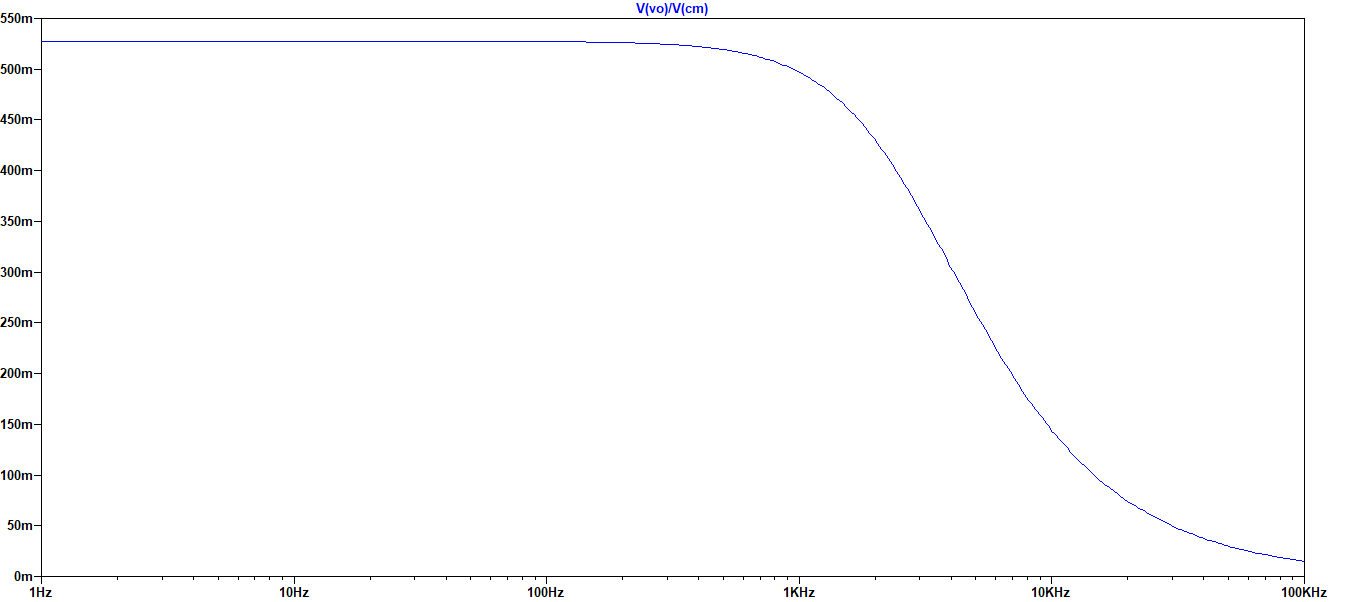
\includegraphics[width=0.9\linewidth]{es1-7-vcm.png}
  	\caption{Guadagno di modo comune complessivo.}
  	\label{fig:gaincm}
\end{figure}

Dai risultati sperimentali possiamo quindi concludere che, a frequenze inferiori rispetto alla frequenza di taglio introdotta (presumibilmente) dal polo del condensatore i due guadagni corrispondono a
\begin{equation*}
A_d = \frac{v_{out}}{v_{id}} = 1845 \frac{V}{V} \qquad \qquad A_{cm} = \frac{v_{out}}{v_{cm}} = 0.527 \frac{V}{V}
\end{equation*}
Possiamo notare che il guadagno differenziale trovato sperimentalmente risulta molto diverso (circa il 50\%) rispetto al guadagnato differenziale calcolato analiticamente. Oltre questo, possiamo osservare che l'amplificatore presenta, dal punto di vista dei guadagni differenziali, prestazioni molto buone (il CMRR calcolato risulta essere 70.88$\,$dB).


\subsection{Applicare un segnale differenziale sinusoidale di ampiezza v$_{id}$ = 1 mV, frequenza 1 kHz e graficare il segnale di uscita risultante}
La caratteristica del segnale in uscita a fronte di un ingresso sinusoidale di ampiezza 1$\,$mV e frequenza 1$\,$kHz è riportata in Figura \ref{fig:outsig}. \\
\begin{figure}[h!]
  	\centering
 	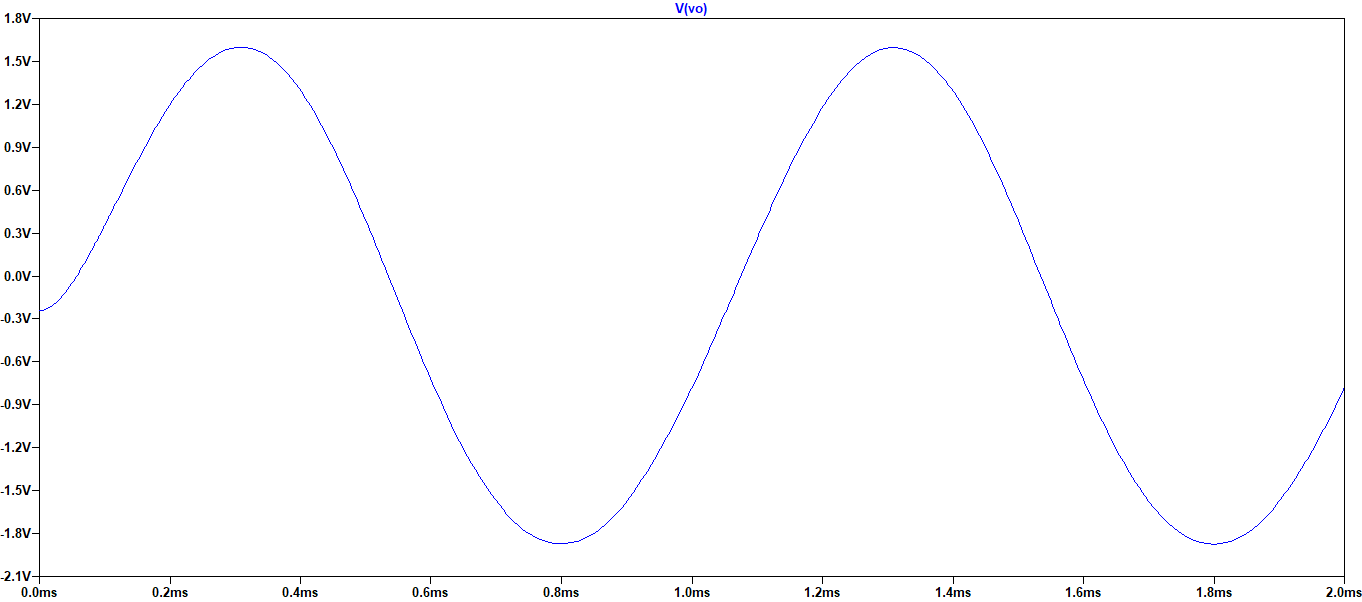
\includegraphics[width=1\linewidth]{es1-8.png}
  	\caption{Segnale in uscita risultante.}
  	\label{fig:outsig}
\end{figure}

Possiamo notare come l'ampiezza del segnale in uscita corrisponda esattamente all'ampiezza del segnale iniziale moltiplicata per il guadagno $A_d$ trovato al punto precedente. Inoltre, il segnale in uscita oscilla con un offset di tensione non nullo, che corrisponde esattamente alla tensione nel punto di lavoro (non calcolabile, ma verificabile sperimentalmente) ai drain dei transistor Q6 e Q7.

\newpage
\section{Esercizio secondo}
Il circuito in Figura genera la somma di A e B e il corrispondente riporto (entrambi negati). Sia $V_{Tn}$ = 0.7$\,$V, k’$_n$ = 160 $\frac{\mu A}{V^2}$, $V_{An}$ = 10$\,$V, $V_{Tp}$=-0.7$\,$V, k’$_p$=40 $\frac{\mu A}{V^2}$. La tensione di alimentazione V$_{DD}$ è di 2.5$\,$V.
\begin{figure}[h!]
  	\centering
 	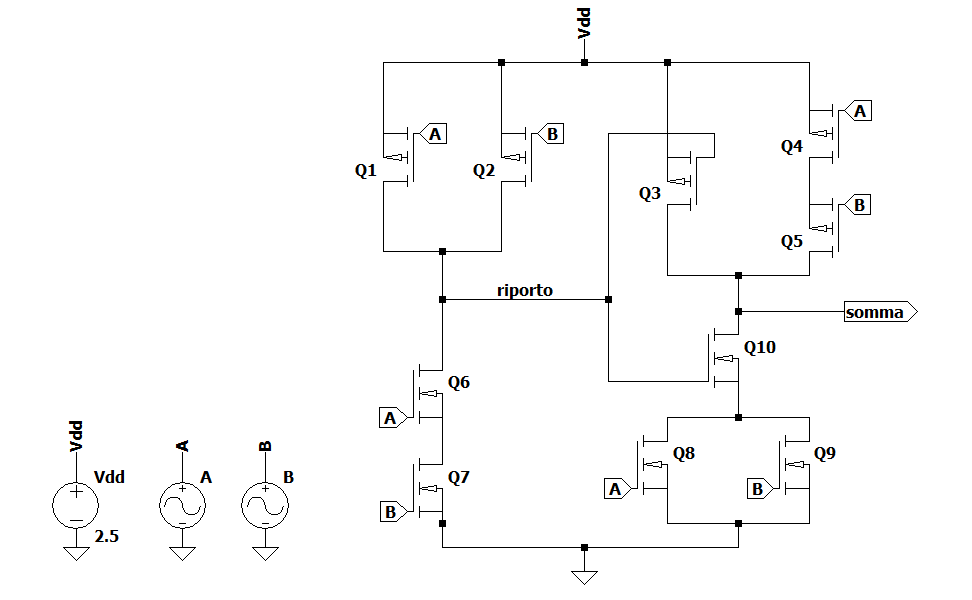
\includegraphics[width=0.7\linewidth]{ckt2.png}
  	\caption{Schema elettrico del sommatore a due bit con riporto.}
  	\label{fig:ckt2}
\end{figure}

\subsection{Identificare somma e riporto, dimensionare W per tutti i transistor in modo che le reti di pull-up e pull-down abbiano la stessa conducibilità e simulare con SPICE la caratteristica DC con B=0, A variabile tra 0 e V$_{DD}$}
Come è già stato evidenziato nello schema circuitale del componente mediante opportune label, l'output del primo stadio costituisce il riporto della somma, mentre l'output del secondo stadio costituisce la somma vera e propria (entrambe negate). Questi risultati derivano direttamente dalle tabelle di verità dei singoli stati, riportate di seguito (Tabella \ref{tabellastad1} e Tabella \ref{tabellastad2}).
\\

\begin{table}[h!]
\begin{center}
\begin{tabular}{ |c|c|c|c|c|c|c| } 
 \hline
   A & B & $Q_{Ap}$ & $Q_{Bp}$ & $Q_{An}$ & $Q_{Bn}$ & $out'$  \\ 
  \hline
   0 & 0 & on & on & off & off & "1" \\ 
   0 & 1 & on & off & off & on & "1" \\ 
   1 & 0 & off & on & on & off & "1" \\ 
   1 & 1 & off & off & on & on & "0" \\ 
 \hline
\end{tabular}
 \caption{Tabella di verità del primo stadio del sommatore.}
\label{tabellastad1}
\end{center}
\end{table}
\begin{table}[h!]
\begin{center}
\begin{tabular}{ |c|c|c|c|c|c|c|c|c|c| } 
 \hline
   A & B & out' & $Q_{Ap}$ & $Q_{Bp}$ & $Q_{op}$ & $Q_{An}$ & $Q_{Bn}$ & $Q_{on}$ & out \\ 
  \hline
   0 & 0 & 1 & on & on & off & off & off & on & "1" \\ 
   0 & 1 & 1 & on & off & off & off & on & on & "0" \\ 
   1 & 0 & 1 & off & on & off & on & off & on & "0" \\ 
   1 & 1 & 0 & off & off & on & on & on & off & "1" \\ 
 \hline
\end{tabular}
 \caption{Tabella di verità del secondo stadio del sommatore.}
\label{tabellastad2}
\end{center}
\end{table}

Il dimensionamento dei transistor deve essere fatto in modo tale che, nel caso peggiore, le reti di pull-up e pull-down abbiano la stessa conducibilità. A partire dalle transconduttanze di processo $k'_n$ e $k'_p$ possiamo trovare il rapporto tra mobilità degli elettroni e mobilità delle lacune e, di conseguenza, il rapporto tra i fattori $\textit{n}$ e $\textit{p}$.
\begin{equation*}
\frac{\mu _n}{\mu _p} = \frac{p}{n} = \frac{k'_n}{k'_p} = 4
\end{equation*}
Possiamo quindi trovare $W_n=0.8\mu m$ e $W_p=3.2\mu m$. I casi peggiori delle singole reti sono:
\begin{itemize}
\item rete di pull-down del primo stadio, è una serie di NMOS e il caso peggiore (nonché l'unico) si verifica quando sono entrambi accesi, dimensione $\textit{2n}$
\item rete di pull-up del primo stadio, è un parallelo di PMOS e il caso peggiore si verifica quando almeno uno dei due è acceso, dimensione $\textit{p}$
\item rete di pull-down del secondo stadio, è una serie tra un NMOS e un parallelo, il caso peggiore si verifica quando ci sono due MOS in serie accesi, dimensione $\textit{2n}$
\item rete di pull-up del secondo stadio, è un parallelo tra un PMOS e una serie di PMOS, il caso peggiore si verifica quando ci sono due MOS accesi, dimensione $\textit{2n}$ nel percorso del caso peggiore
\end{itemize}
Il circuito che ne risulta è il seguente, riportato in Figura \ref{fig:dimensionamento}.
\begin{figure}[h!]
  	\centering
 	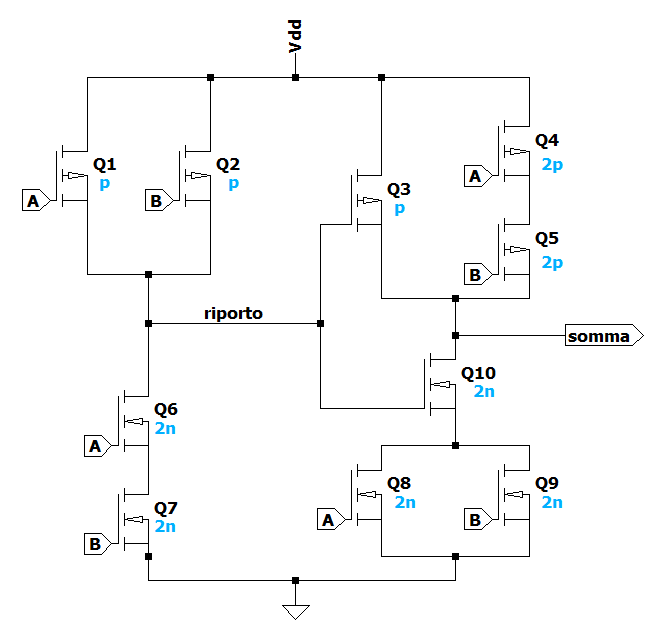
\includegraphics[width=0.7\linewidth]{es2-dimens.png}
  	\caption{Dimensionamento transistor.}
  	\label{fig:dimensionamento}
\end{figure}
\newpage
\noindent Per simulare la caratteristica di trasferimento sul parametro A è stato utilizzato il seguente listato SPICE. Il risultato della simulazione è riportato in Figura \ref{fig:somm1}. 
\small
\begin{quote}
\begin{verbatim}
* Esercizio 2
* pull-up riporto
M1 riporto A Vdd Vdd PMOS
M2 riporto B Vdd Vdd PMOS
* pull-down riporto
M6 riporto A N3 0 NMOS2
M7 N3 B 0 0 NMOS2
* pull-up somma
M3 somma riporto Vdd Vdd PMOS
M4 N1 A Vdd Vdd PMOS2
M5 somma B N1 Vdd PMOS2
* pull-down somma
M10 somma riporto N2 0 NMOS2
M8 N2 A 0 0 NMOS2
M9 N2 B 0 0 NMOS2
* Vdd e segnali
Vdd Vdd 0 2.5
Va A 0 {in}
Vb B 0 0
.model NMOS NMOS LEVEL=1 VTO=0.7 KP=160u W=0.8u L=0.8u LAMBDA=0.1
.model NMOS2 NMOS LEVEL=1 VTO=0.7 KP=160u W=1.6u L=0.8u LAMBDA=0.1
.model PMOS PMOS LEVEL=1 VTO=-0.7 KP=40u W=3.2u L=0.8u LAMBDA=0.1
.model PMOS2 PMOS LEVEL=1 VTO=-0.7 KP=40u W=6.4u L=0.8u LAMBDA=0.1
.dc param in 0 2.5 10m
.backanno
.end
\end{verbatim}
\end{quote}
\normalsize
\begin{figure}[h!]
  	\centering
 	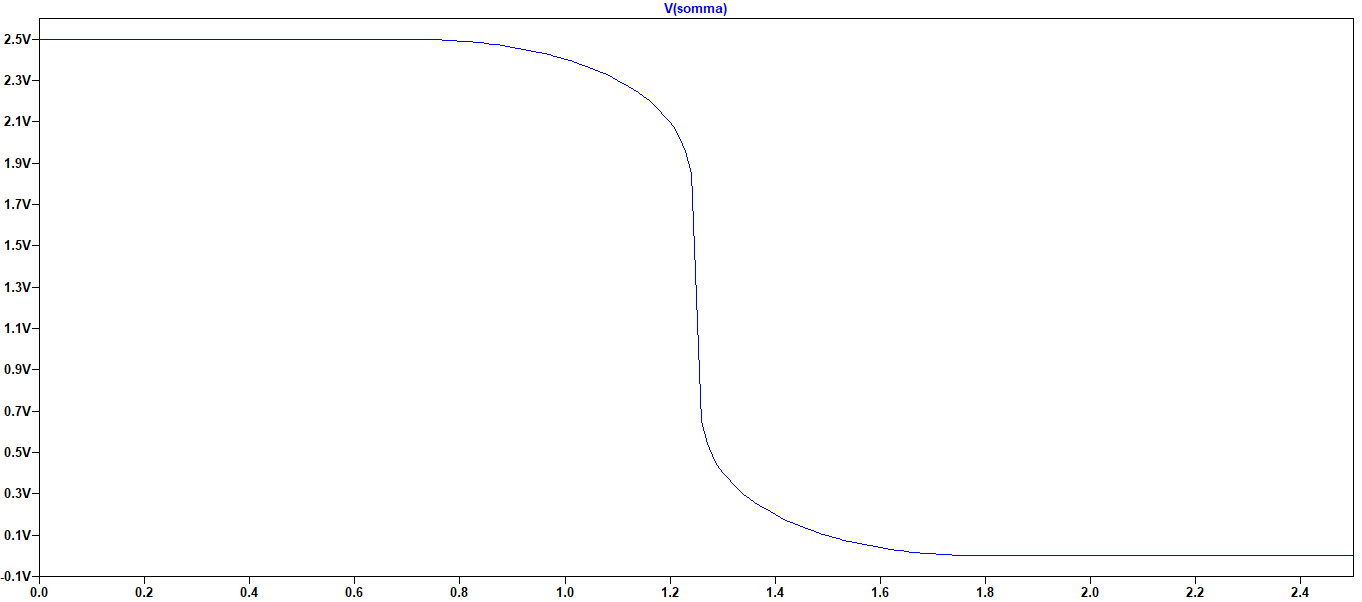
\includegraphics[width=1\linewidth]{es2-1-somma.png}
  	\caption{Risposta del sommatore in funzione del valore della tensione A, B nullo.}
  	\label{fig:somm1}
\end{figure}
Il circuito sommatore, secondo quanto riportato in Figura \ref{fig:somm1}, risulta quindi essere bilanciato. La variazione della caratteristica d'uscita, studiata al variare di uno dei due ingressi, risulta avvenire infatti per un valore esattamente pari a $\frac{V_{DD}}{2}$.
\newpage

\subsection{Applicare all'uscita della somma un condensatore da $100\,$fF, e calcolare la potenza dissipata in uscita nel caso AB commutino simultaneamente da 10 a 00 a 10 con una frequenza di clock pari al proprio numero di matricola}
La transizione 10$\rightarrow$00$\rightarrow$10 agli ingressi AB del sommatore causa una variazione LOW-HIGH-LOW all'uscita del secondo stadio, mentre l'output del primo stadio rimane inalterato (costante al valore "1"). Pertanto la potenza dissipata in uscita durante l'intero ciclo può essere calcolata come
\begin{equation*}
P_{dyn}=C_L\cdot V_{DD}^2 \cdot f = 742\,nW
\end{equation*}
Per misurare la potenza dissipata nel ciclo L-H-L dal circuito modifichiamo il segnale in ingresso in modo che abbia frequenza pari al numero di matricola (e quindi periodo $T=\frac{1}{f}$).
\begin{quote}
\begin{verbatim}
Va A 0 PULSE(0 2.5 1f 1f 1f 280.078n 561.555n)
\end{verbatim}
\end{quote}
La potenza misurata sperimentalmente con SPICE coincide, a meno di un errore pari a circa il 2.5\%, con la potenza precedentemente calcolata. Il risultato della simulazione è riportato in Figura \ref{fig:powerso}.

\begin{figure}[h!]
  	\centering
 	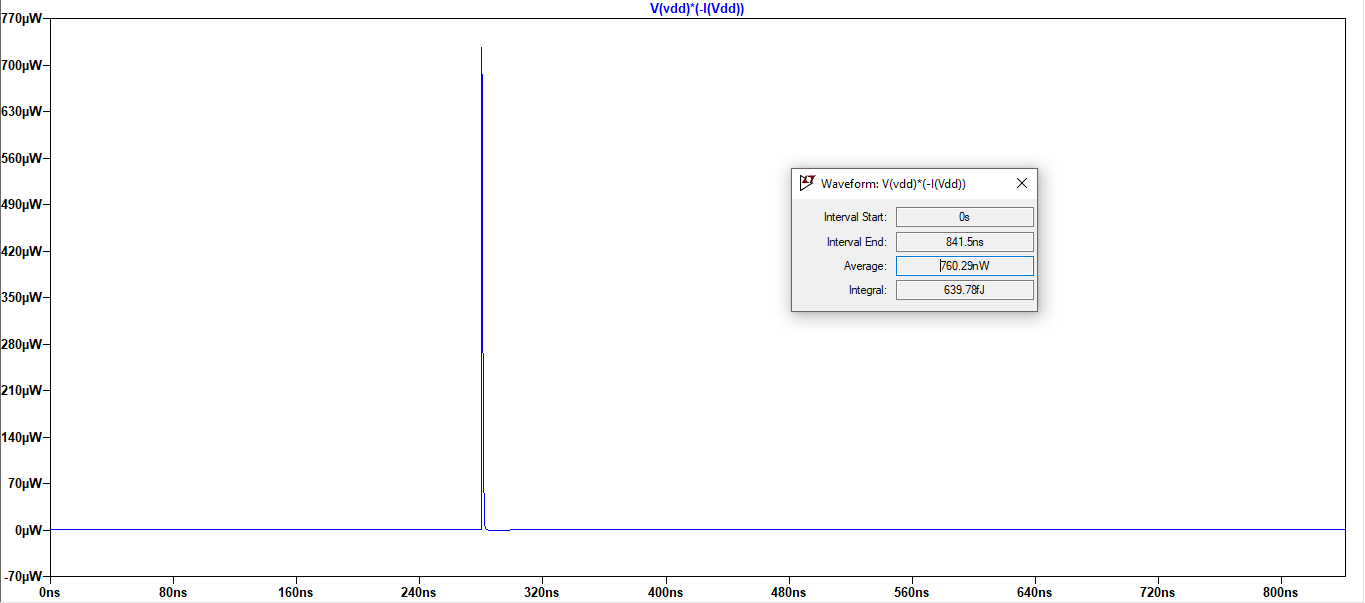
\includegraphics[width=1\linewidth]{es2-2power.png}
  	\caption{Potenza dissipata nel sommatore.}
  	\label{fig:powerso}
\end{figure}
\newpage

\subsection{Mantenere B=0 e simulare con SPICE il transitorio di uscita della somma negata con A che commuta tra 0 e 1 con e senza carico capacitivo}
Il listato SPICE utilizzato per simulare il transitorio in uscita della somma negata con A che commuta tra 0 e 1 (mentre B rimane costante a 0) è lo stesso riportato nel punto precedente, con l'unica differenza che il segnale di ingresso A diventa un segnale ad onda quadra di frequenza 5$\,$MHz come riportato di seguito
\small
\begin{quote}
\begin{verbatim}
Va A 0 PULSE(0 2.5 1p 1p 1p 100n 200n)
\end{verbatim}
\end{quote}
\normalsize
Inoltre, è stata aggiunta anche una capacità di carico C$_1$ il cui valore è parametrizzato e $\in$ {0,100$\,$fF}. Con questo stratagemma è stato possibile plottare contemporaneamente le caratteristiche dell'uscita con e senza capacità di carico (\small \textit{i grafici di colore blu rappresentano il comportamento senza capacità, quelli di colore rosso invece il comportamento con capacità collegata} \normalsize).
\small
\begin{quote}
\begin{verbatim}
C1 somma 0 {cap}
.step param cap 0 100f 100f
.tran 0 300n
\end{verbatim}
\end{quote}
\normalsize
L'analisi è stata fatta sul comportamento transitorio in un periodo e mezzo del segnale in ingresso (corrispondente ad un ciclo LOW-HIGH-LOW dell'uscita). I risultati della simulazione sono riportati in Figura \ref{fig:carica31} e Figura \ref{fig:scarica32}. 
\begin{figure}[h!]
  	\centering
 	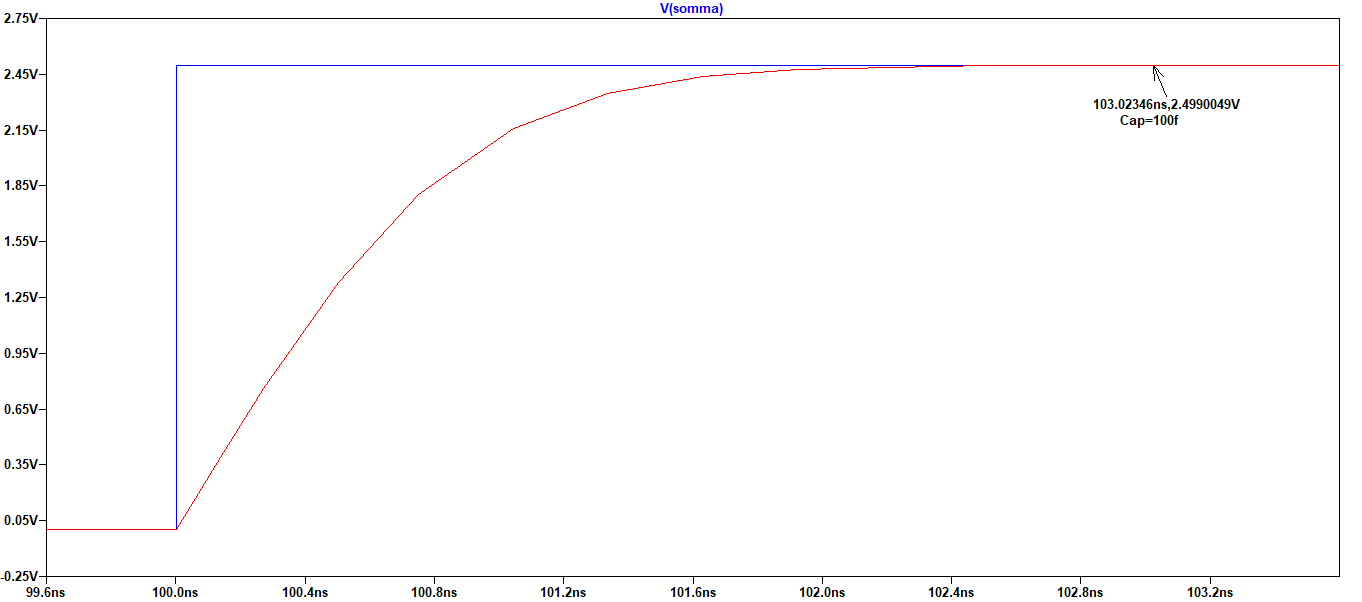
\includegraphics[width=0.9\linewidth]{es2-3-carica.png}
  	\caption{Commutazione ingresso a 1$\rightarrow$0.}
  	\label{fig:carica31}
\end{figure}
\begin{figure}[h!]
  	\centering
 	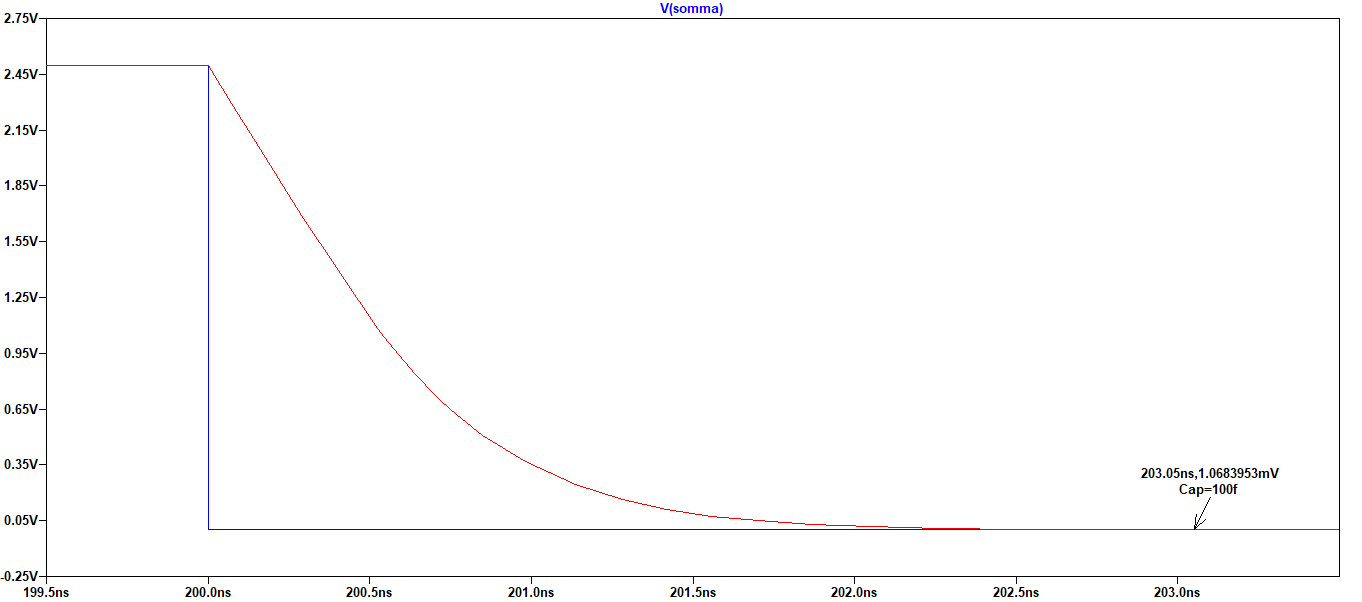
\includegraphics[width=0.9\linewidth]{es2-3-scarica.png}
  	\caption{Commutazione ingresso a 0$\rightarrow$1.}
  	\label{fig:scarica32}
\end{figure}

\noindent Notiamo come i tempi di salita e discesa in commutazione siamo approssimativamente gli stessi ($\approx3\,ns$).

\newpage
\subsection{Ripetere il punto 2.3 dimensionando tutti i transistor con W=6.4$\mu$m, L=0.8$\mu$m. Cosa cambia? Perché?}
Innanzitutto, modifichiamo i valori di W e L nella simulazione SPICE come di seguito
\begin{quote}
\begin{verbatim}
.model NMOS NMOS LEVEL=1 VTO=0.7 KP=160u W=6.4u L=0.8u LAMBDA=0.1
.model NMOS2 NMOS LEVEL=1 VTO=0.7 KP=160u W=6.4u L=0.8u LAMBDA=0.1
.model PMOS PMOS LEVEL=1 VTO=-0.7 KP=40u W=6.4u L=0.8u LAMBDA=0.1
.model PMOS2 PMOS LEVEL=1 VTO=-0.7 KP=40u W=6.4u L=0.8u LAMBDA=0.1
\end{verbatim}
\end{quote}
Il risultato della simulazione, osservati con una scala dei tempi molto dilatata in modo tale da poter apprezzare il comportamento nel transitorio, è riportato in Figura \ref{fig:carica41} e Figura \ref{fig:scarica42}.\\
\begin{figure}[h!]
  	\centering
 	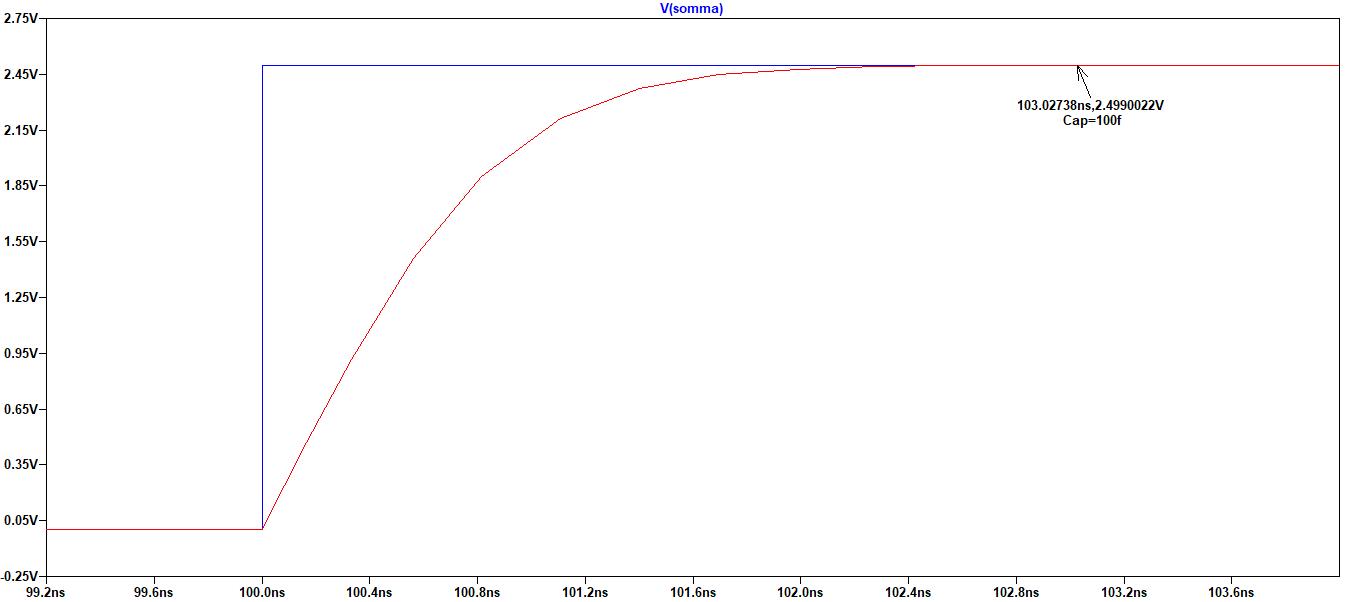
\includegraphics[width=0.9\linewidth]{es2-4-carica.png}
  	\caption{Commutazione ingresso a 1$\rightarrow$0.}
  	\label{fig:carica41}
\end{figure}
\begin{figure}[h!]
  	\centering
 	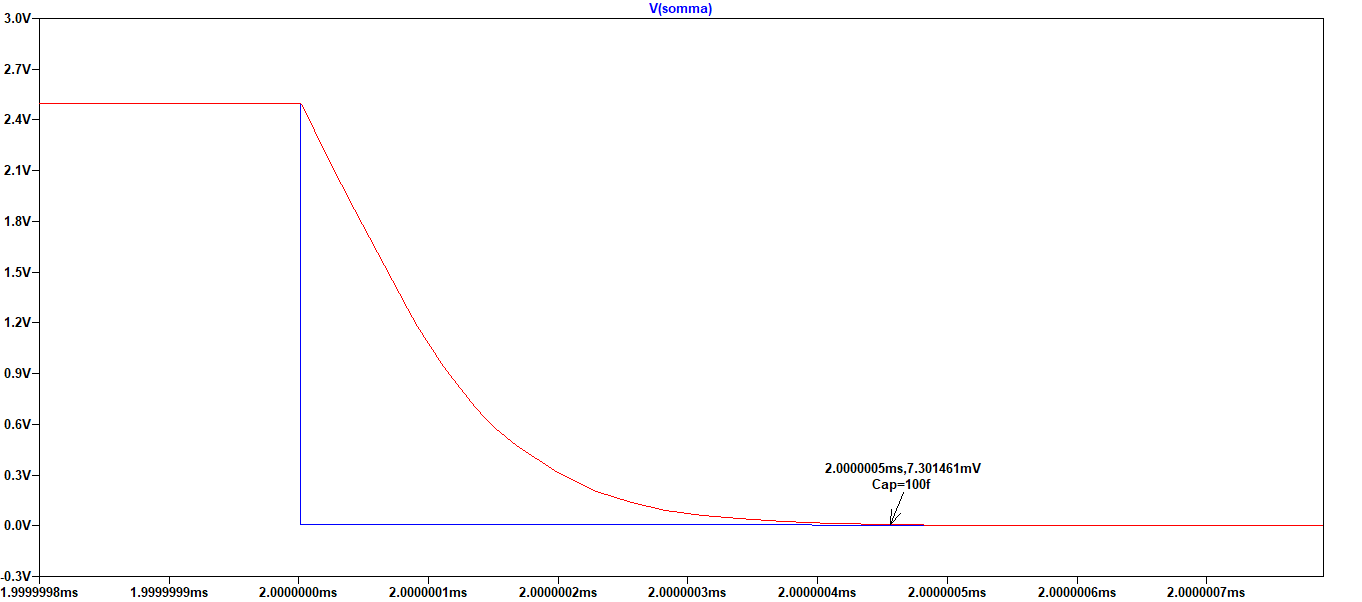
\includegraphics[width=0.9\linewidth]{es2-4-scarica.png}
  	\caption{Commutazione ingresso a 0$\rightarrow$1.}
  	\label{fig:scarica42}
\end{figure}\\

Possiamo notare come, a differenza del caso precedente, i tempi di salita e discesa dell'uscita che rappresenta la somma negata (rispettivamente 3.028$\,$ns e 0.601$\,$ns per raggiungere il valore di uscita ideale $\pm$1$\,$mV) siano tra loro molto diversi. Questa differenza così accentuata è causata dalla minor conduttività delle lacune rispetto agli elettroni, che rende molto più veloce lo scarica attraverso i transistor NMOS (il cui canale è formato da elettroni) piuttosto che la carica attraverso i PMOS (il cui canale è invece formato da lacune).
\end{document}